\newpage
\section{Metodologia Experimental}

\subsection{Materiais}
O material utilizado foi:
\begin{itemize}
\item Computador.
\item Software Orcad.
\end{itemize}

\subsection{Métodos}

\subsubsection{Redes Adaptadoras de Banda Estreita: 2 e 3 elementos (L, T e $\pi$)}

1- A partir do circuito da figura \ref{fig:redeL}, projetar uma rede adaptadora de impedância com 2 elementos (rede L) tal que $Z_{in} = 50 \ \Omega$ em $\omega_0 = 4300 krad/s$; com impedância de saída $Z_{out} = 1k\Omega$. Admita que a rede tenha também a função de bloquear a eventual componente DC a fonte.

\begin{figure}[H]
    \centering
    \caption{Rede L.}
    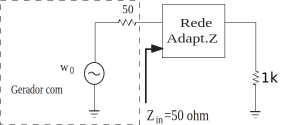
\includegraphics[scale=1]{Imagens/redeL.pdf}
    \label{fig:redeL}
    
    \small Fonte: Me. Jaime Laelson Jacob, 2016.
\end{figure}

\begin{enumerate}[label=\alph*]
    \item Montar o circuito com a rede adaptadora projetada;
    
    \item Injetar um sinal senoidal de frequência $\omega_0$ e
    amplitude da ordem de centenas de milivolts de pico na entrada do circuito montado.
    
    \item Observar a forma de onda da entrada, sobre a carga à saída e sobre a carga resistiva à saída. Anotar as formas de onda.
    
    \item Variar a frequência do sinal senoidal até obter o perfeito casamento de impedância entre fonte e carga. Anotar esta frequência.
    
    \item Obter o índice de mérito do circuito completo ($Q_{Load}$). Calcular este paramento e comparar com o medido. Obter a banda de passagem da rede adotando um dos critérios para adaptação de impedância, sintetizados nas equações (6) e (7).
   \end{enumerate} 

2- Reprojetar a rede adaptadora utilizando 3 elementos (rede T ou $\pi$). Admita agora que não há restrição para o bloqueio de eventuais componentes
DC entre fonte e carga.
\begin{enumerate}[label=\alph*]
    \item Variar a frequência do sinal senoidal até obter o perfeito casamento de impedância entre fonte e carga. Anotar esta frequência.
    
    \item  Obter, através de um procedimento experimental, o novo índice de mérito carregado para a rede de 3 elementos. Comparar com o valor teórico do projeto.
    
    \item Qual a banda de passagem para esta topologia. Adote o mesmo critério utilizado anteriormente.
\end{enumerate}


\subsubsection{Rede Adaptadora de Banda Larga (WBand)}

A partir do problema de adaptação de impedância mostrado na figura 2, calcular e implementar uma rede de banda larga de 2 seções L de tal forma a maximizar a banda de passagem. Nesta condição, calcular o índice de qualidade carregado do circuito. Como frequência central de projeto, adote a mesma do item anterior.

Passos experimentais:
\begin{enumerate}[label=\alph*]
    \item Montar o circuito com a rede adaptadora WBand projetada.
    
    \item  Obter a BW da rede adotando o mesmo critério utilizado anteriormente na obtenção da BW da rede de banda estreita. Comparar o incremento na BW com relação ao caso anterior.
    
    \item Medir o $Q_{rede}$ WBand e comparar com o valor teórico.
\end{enumerate}

